\documentclass[9pt,a4paper,]{extarticle}

\usepackage{f1000_styles}

\usepackage[pdfborder={0 0 0}]{hyperref}

\usepackage[numbers]{natbib}
\bibliographystyle{unsrtnat}


%% maxwidth is the original width if it is less than linewidth
%% otherwise use linewidth (to make sure the graphics do not exceed the margin)
\makeatletter
\def\maxwidth{ %
  \ifdim\Gin@nat@width>\linewidth
    \linewidth
  \else
    \Gin@nat@width
  \fi
}
\makeatother

\usepackage{color}
\usepackage{fancyvrb}
\newcommand{\VerbBar}{|}
\newcommand{\VERB}{\Verb[commandchars=\\\{\}]}
\DefineVerbatimEnvironment{Highlighting}{Verbatim}{commandchars=\\\{\}}
% Add ',fontsize=\small' for more characters per line
\usepackage{framed}
\definecolor{shadecolor}{RGB}{248,248,248}
\newenvironment{Shaded}{\begin{snugshade}}{\end{snugshade}}
\newcommand{\AlertTok}[1]{\textcolor[rgb]{0.94,0.16,0.16}{#1}}
\newcommand{\AnnotationTok}[1]{\textcolor[rgb]{0.56,0.35,0.01}{\textbf{\textit{#1}}}}
\newcommand{\AttributeTok}[1]{\textcolor[rgb]{0.13,0.29,0.53}{#1}}
\newcommand{\BaseNTok}[1]{\textcolor[rgb]{0.00,0.00,0.81}{#1}}
\newcommand{\BuiltInTok}[1]{#1}
\newcommand{\CharTok}[1]{\textcolor[rgb]{0.31,0.60,0.02}{#1}}
\newcommand{\CommentTok}[1]{\textcolor[rgb]{0.56,0.35,0.01}{\textit{#1}}}
\newcommand{\CommentVarTok}[1]{\textcolor[rgb]{0.56,0.35,0.01}{\textbf{\textit{#1}}}}
\newcommand{\ConstantTok}[1]{\textcolor[rgb]{0.56,0.35,0.01}{#1}}
\newcommand{\ControlFlowTok}[1]{\textcolor[rgb]{0.13,0.29,0.53}{\textbf{#1}}}
\newcommand{\DataTypeTok}[1]{\textcolor[rgb]{0.13,0.29,0.53}{#1}}
\newcommand{\DecValTok}[1]{\textcolor[rgb]{0.00,0.00,0.81}{#1}}
\newcommand{\DocumentationTok}[1]{\textcolor[rgb]{0.56,0.35,0.01}{\textbf{\textit{#1}}}}
\newcommand{\ErrorTok}[1]{\textcolor[rgb]{0.64,0.00,0.00}{\textbf{#1}}}
\newcommand{\ExtensionTok}[1]{#1}
\newcommand{\FloatTok}[1]{\textcolor[rgb]{0.00,0.00,0.81}{#1}}
\newcommand{\FunctionTok}[1]{\textcolor[rgb]{0.13,0.29,0.53}{\textbf{#1}}}
\newcommand{\ImportTok}[1]{#1}
\newcommand{\InformationTok}[1]{\textcolor[rgb]{0.56,0.35,0.01}{\textbf{\textit{#1}}}}
\newcommand{\KeywordTok}[1]{\textcolor[rgb]{0.13,0.29,0.53}{\textbf{#1}}}
\newcommand{\NormalTok}[1]{#1}
\newcommand{\OperatorTok}[1]{\textcolor[rgb]{0.81,0.36,0.00}{\textbf{#1}}}
\newcommand{\OtherTok}[1]{\textcolor[rgb]{0.56,0.35,0.01}{#1}}
\newcommand{\PreprocessorTok}[1]{\textcolor[rgb]{0.56,0.35,0.01}{\textit{#1}}}
\newcommand{\RegionMarkerTok}[1]{#1}
\newcommand{\SpecialCharTok}[1]{\textcolor[rgb]{0.81,0.36,0.00}{\textbf{#1}}}
\newcommand{\SpecialStringTok}[1]{\textcolor[rgb]{0.31,0.60,0.02}{#1}}
\newcommand{\StringTok}[1]{\textcolor[rgb]{0.31,0.60,0.02}{#1}}
\newcommand{\VariableTok}[1]{\textcolor[rgb]{0.00,0.00,0.00}{#1}}
\newcommand{\VerbatimStringTok}[1]{\textcolor[rgb]{0.31,0.60,0.02}{#1}}
\newcommand{\WarningTok}[1]{\textcolor[rgb]{0.56,0.35,0.01}{\textbf{\textit{#1}}}}

% disable code chunks background
%\renewenvironment{Shaded}{}{}

% disable section numbers
\setcounter{secnumdepth}{0}

%% added by MLS, this is not in the F1000 style by default %%

\hypersetup{unicode=true,
            pdftitle={F1000Research Software Tool Article Template},
            pdfkeywords={Please list up to eight keywords to help readers interested in your article find it more easily.},
            pdfborder={0 0 0},
            breaklinks=true}

%% End added by MLS %%

\setlength{\parindent}{0pt}
\setlength{\parskip}{6pt plus 2pt minus 1pt}



\begin{document}
\pagestyle{front}

\title{\emph{F1000Research} Software Tool Article Template}

%% AUTH AFFIL %%

\maketitle
\thispagestyle{front}

\begin{abstract}
Abstracts should be up to 300 words and provide a succinct summary of the article. Although the abstract should explain why the article might be interesting, care should be taken not to inappropriately over-emphasise the importance of the work described in the article. Citations should not be used in the abstract, and the use of abbreviations should be minimized.
\end{abstract}

\section*{Keywords}
Please list up to eight keywords to help readers interested in your article find it more easily.


\clearpage
\pagestyle{main}

\textbf{R version}: R version 4.3.0 (2023-04-21)

\textbf{Bioconductor version}: 3.17

\hypertarget{introduction}{%
\section{Introduction}\label{introduction}}

The introduction provides context as to why the software tool was developed and what need it addresses. It is good scholarly practice to mention previously developed tools that address similar needs, and why the current tool is needed.

\hypertarget{methods}{%
\section{Methods}\label{methods}}

\hypertarget{implementation}{%
\subsection{Implementation}\label{implementation}}

For software tool papers, this section should address how the tool works and any relevant technical details required for implementation of the tool by other developers.

\hypertarget{operation}{%
\subsection{Operation}\label{operation}}

This part of the methods should include the minimal system requirements needed to run the software and an overview of the workflow for the tool for users of the tool.

\hypertarget{results}{%
\section{\texorpdfstring{Results }{Results }}\label{results}}

This section is only required if the paper includes novel data or analyses, and should be written as a traditional results section.

\hypertarget{use-cases}{%
\section{\texorpdfstring{Use Cases }{Use Cases }}\label{use-cases}}

This section is required if the paper does not include novel data or analyses.
Examples of input and output files should be provided with some explanatory context. Any novel or complex variable parameters should also be explained in sufficient detail to allow users to understand and use the tool's functionality.

\hypertarget{discussion}{%
\section{\texorpdfstring{Discussion }{Discussion }}\label{discussion}}

This section is only required if the paper includes novel data or analyses, and should be written in the same style as a traditional discussion section.
Please include a brief discussion of allowances made (if any) for controlling bias or unwanted sources of variability, and the limitations of any novel datasets.

\hypertarget{conclusions}{%
\section{\texorpdfstring{Conclusions }{Conclusions }}\label{conclusions}}

This section is only required if the paper includes novel data or analyses, and should be written as a traditional conclusion.

\hypertarget{summary}{%
\section{\texorpdfstring{Summary }{Summary }}\label{summary}}

This section is required if the paper does not include novel data or analyses. It allows authors to briefly summarize the key points from the article.

\hypertarget{data-availability}{%
\section{\texorpdfstring{Data availability }{Data availability }}\label{data-availability}}

Please add details of where any datasets that are mentioned in the paper, and that have not have not previously been formally published, can be found. If previously published datasets are mentioned, these should be cited in the references, as per usual scholarly conventions.

\hypertarget{software-availability}{%
\section{Software availability}\label{software-availability}}

This section will be generated by the Editorial Office before publication. Authors are asked to provide some initial information to assist the Editorial Office, as detailed below.

\begin{enumerate}
\def\labelenumi{\arabic{enumi}.}
\tightlist
\item
  URL link to where the software can be downloaded from or used by a non-coder (AUTHOR TO PROVIDE; optional)
\item
  URL link to the author's version control system repository containing the source code (AUTHOR TO PROVIDE; required)
\item
  Link to source code as at time of publication (\emph{F1000Research} TO GENERATE)
\item
  Link to archived source code as at time of publication (\emph{F1000Research} TO GENERATE)
\item
  Software license (AUTHOR TO PROVIDE; required)
\end{enumerate}

\hypertarget{author-information}{%
\section{Author information}\label{author-information}}

In order to give appropriate credit to each author of an article, the individual contributions of each author to the manuscript should be detailed in this section. We recommend using author initials and then stating briefly how they contributed.

\hypertarget{competing-interests}{%
\section{Competing interests}\label{competing-interests}}

All financial, personal, or professional competing interests for any of the authors that could be construed to unduly influence the content of the article must be disclosed and will be displayed alongside the article. If there are no relevant competing interests to declare, please add the following: `No competing interests were disclosed'.

\hypertarget{grant-information}{%
\section{Grant information}\label{grant-information}}

Please state who funded the work discussed in this article, whether it is your employer, a grant funder etc. Please do not list funding that you have that is not relevant to this specific piece of research. For each funder, please state the funder's name, the grant number where applicable, and the individual to whom the grant was assigned. If your work was not funded by any grants, please include the line: `The author(s) declared that no grants were involved in supporting this work.'

\hypertarget{acknowledgments}{%
\section{Acknowledgments}\label{acknowledgments}}

This section should acknowledge anyone who contributed to the research or the article but who does not qualify as an author based on the criteria provided earlier (e.g.~someone or an organization that provided writing assistance). Please state how they contributed; authors should obtain permission to acknowledge from all those mentioned in the Acknowledgments section.

Please do not list grant funding in this section.

\hypertarget{using-r-markdown}{%
\section{USING R MARKDOWN}\label{using-r-markdown}}

Some examples of commonly used markdown syntax are listed below, to help you get started.

\hypertarget{cross-references}{%
\subsection{Cross-references}\label{cross-references}}

For portability between different output formats, use the syntax introduced by \emph{bookdown}, such as \texttt{(\textbackslash{}\#label)} for labels and \texttt{\textbackslash{}@ref(label)} for cross-references. The following sections provide examples of referencing tables, figures, and equations.

\hypertarget{citations}{%
\subsection{Citations}\label{citations}}

You can include references in a standard Bibtex file. The name of this file is given in the header of the markdown document (in our case it is \emph{sample.bib}). References to entries in the Bibtex file are made using square brackets and use an @ plus the key for the entry you are referencing \citep{Smith:2012qr}. You can combine multiple entries by separating them with a semi-colon \citep{Smith:2012qr, Smith:2013jd}.
The default bibliography style uses numerical citations. For superscript or author-year citations set the header metadata field \texttt{natbiboptions} to either \texttt{super} or \texttt{round}, respectively.

\hypertarget{code-chunks}{%
\subsection{Code chunks}\label{code-chunks}}

You can embed an R code chunk like this:

\begin{Shaded}
\begin{Highlighting}[]
\NormalTok{x }\OtherTok{\textless{}{-}} \DecValTok{1}\SpecialCharTok{:}\DecValTok{10}
\NormalTok{x}
\end{Highlighting}
\end{Shaded}

\begin{verbatim}
##  [1]  1  2  3  4  5  6  7  8  9 10
\end{verbatim}

If you specify a figure caption to a code chunk using the chunk option \texttt{fig.cap}, the plot will be automatically labeled and numbered. The figure label is generated from the label of the code chunk by prefixing it with \texttt{fig:}, e.g., see Figure @ref(fig:plot).

\begin{Shaded}
\begin{Highlighting}[]
\FunctionTok{plot}\NormalTok{(x)}
\end{Highlighting}
\end{Shaded}

\begin{figure}

{\centering 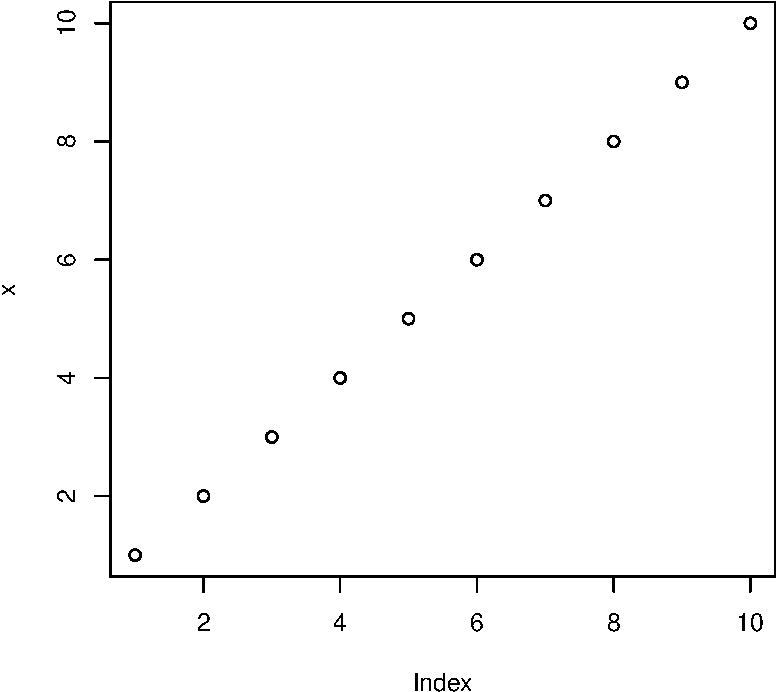
\includegraphics[width=0.6\linewidth]{RMeDPower_vignette_files/figure-latex/plot-1} 

}

\caption{A caption to our sample plot.}(\#fig:plot)
\end{figure}

\hypertarget{tables}{%
\subsection{Tables}\label{tables}}

Markdown syntax tends to lack some of the more sophisticated formatting features available in LaTeX, so you may need to edit the tables later to get the desired format.

\begin{longtable}[]{@{}lll@{}}
\caption{Caption to table.}\tabularnewline
\toprule\noalign{}
First name & Last Name & Grade \\
\midrule\noalign{}
\endfirsthead
\toprule\noalign{}
First name & Last Name & Grade \\
\midrule\noalign{}
\endhead
\bottomrule\noalign{}
\endlastfoot
John & Doe & 7.5 \\
Richard & Miles & 2 \\
\end{longtable}

Just like figures, tables with captions will also be numbered and can be referenced. Captions are entered as a paragraph beginning with the string ``Table:'' (or just ``:''), which may appear either before or after the table. A label for the table should appear in the beginning of the caption in the form of \texttt{(\textbackslash{}\#tab:label)}, e.g., see Table @ref(tab:table).

\begin{longtable}[]{@{}lcr@{}}
\caption{(\#tab:table) A table with text justification.}\tabularnewline
\toprule\noalign{}
First name & Last Name & Grade \\
\midrule\noalign{}
\endfirsthead
\toprule\noalign{}
First name & Last Name & Grade \\
\midrule\noalign{}
\endhead
\bottomrule\noalign{}
\endlastfoot
John & Doe & 7.5 \\
Richard & Miles & 2 \\
\end{longtable}

\hypertarget{figures}{%
\subsection{Figures}\label{figures}}

You can include static figures (i.e.~no generated by code) using the \texttt{include\_graphics()} function from the \textbf{knitr} package, in a standard code chunk.

\begin{Shaded}
\begin{Highlighting}[]
\NormalTok{knitr}\SpecialCharTok{::}\FunctionTok{include\_graphics}\NormalTok{(}\StringTok{\textquotesingle{}frog.jpg\textquotesingle{}}\NormalTok{, }\AttributeTok{error =} \ConstantTok{FALSE}\NormalTok{)}
\end{Highlighting}
\end{Shaded}

\begin{figure}

{\centering 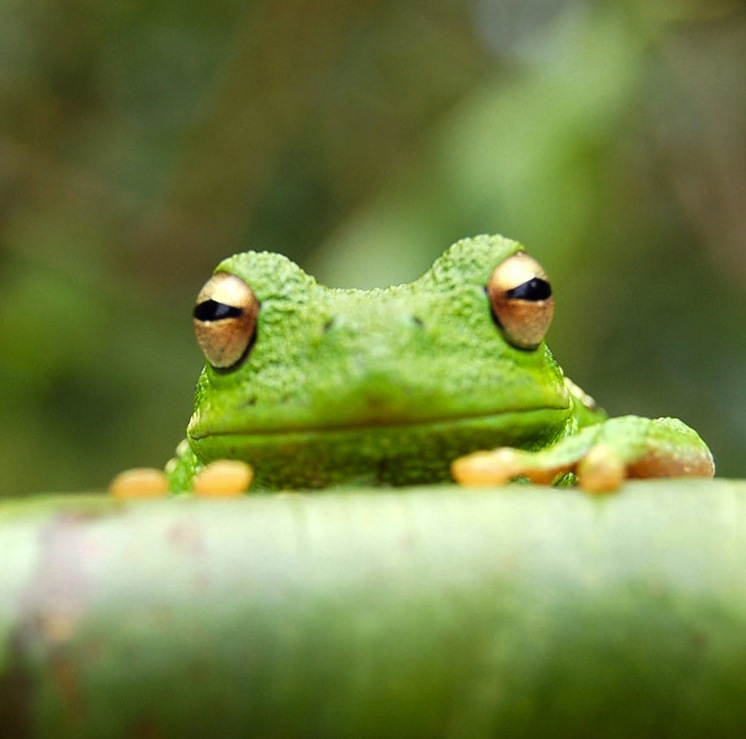
\includegraphics[width=0.5\linewidth]{frog} 

}

\caption{Your figure legend goes here; it should be succinct, while still explaining all symbols and abbreviations.}(\#fig:frog-picture)
\end{figure}

You can again use the \texttt{fig.cap} option to provide the figure caption, and reference the image based on the code chunk label. You can also use options such as \texttt{fig.align} and \texttt{fig.width} to adjust the position and size of the image within the final document, e.g.~Figure @ref(fig:frog-picture) is a frog.

Alternatively, you can use the standard markdown syntax like so:

\begin{figure}
\centering
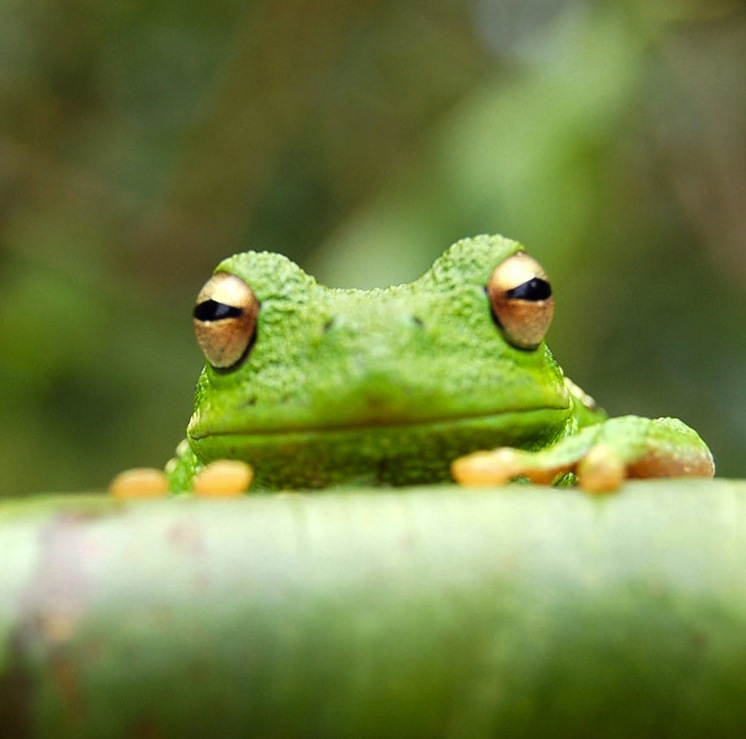
\includegraphics[width=2cm,height=2cm]{frog.jpg}
\caption{This is a smaller version of the same picture, inserted using the standard markdown syntax}
\end{figure}

Please give figures appropriate filenames, e.g.: figure1.pdf, figure2.png.

Figure legends should briefly describe the key messages of the figure such that the figure can stand alone from the main text. However, all figures should also be discussed in the article text. Each legend should have a concise title of no more than 15 words. The legend itself should be succinct, while still explaining all symbols and abbreviations. Avoid lengthy descriptions of methods.

For any figures reproduced from another publication (as long as appropriate permission has been obtained from the copyright holder -see under the heading `Submission'), please include a line in the legend to state that: `This figure has been reproduced with kind permission from {[}include original publication citation{]}'.

\hypertarget{mathematics}{%
\subsection{Mathematics}\label{mathematics}}

You can use LaTeX syntax to typeset mathematical expressions. Let \(X_1, X_2, \ldots, X_n\) be a sequence of independent and identically distributed random variables with \(\text{E}[X_i] = \mu\) and \(\text{Var}[X_i] = \sigma^2 < \infty\), and let
\[S_n = \frac{X_1 + X_2 + \cdots + X_n}{n}
      = \frac{1}{n}\sum_{i}^{n} X_i\]
denote their mean. Then as \(n\) approaches infinity, the random variables \(\sqrt{n}(S_n - \mu)\) converge in distribution to a normal \(\mathcal{N}(0, \sigma^2)\).

To number and refer to equations, put them in the equation environments and assign labels to them, as for Equation @ref(eq:binom).

\begin{equation}
  f\left(k\right) = \binom{n}{k} p^k\left(1-p\right)^{n-k}
  (\#eq:binom)
\end{equation}

\hypertarget{lists}{%
\subsection{Lists}\label{lists}}

You can make ordered lists

\begin{enumerate}
\def\labelenumi{\arabic{enumi}.}
\tightlist
\item
  Like this,
\item
  and like this.
\end{enumerate}

or bullet points

\begin{itemize}
\tightlist
\item
  Like this,
\item
  and like this.

  \begin{itemize}
  \tightlist
  \item
    Use indentation

    \begin{itemize}
    \tightlist
    \item
      for sub-items
    \end{itemize}
  \end{itemize}
\end{itemize}

\hypertarget{additional-advice-to-authors}{%
\section{Additional advice to authors}\label{additional-advice-to-authors}}

The content above is either taken directly from the F1000Research \LaTeX~template, or has been adpated to suit R Markdown. Here we provide some additional advice to authors based on our own and other users' experiences of article submission to F1000Research, which will hopefully make your own journey smoother. If you would like to contribute to this, please contact us at \url{https://github.com/grimbough/BiocWorkflowTools/issues/4}

\begin{itemize}
\tightlist
\item
  When writing figure or tables captions do not use acronyms or abbreviations without explanation in the legend itself, even this has been addressed in the main text. F1000Research require each figure and table to be able to stand alone from the rest of the manuscript. \emph{Thanks to Mike Love \href{https://twitter.com/mikelove}{@mikelove}}
\end{itemize}

{\small\bibliography{sample.bib}}

\end{document}
